\documentclass[a4paper,12pt]{article}

% Preamble
\usepackage{amsmath}
\usepackage[english,russian]{babel}
\usepackage{graphicx}
\usepackage[utf8]{inputenc}
\usepackage{indentfirst}
\usepackage[T2A]{fontenc}
\usepackage{tabularx}
\usepackage{textcomp}
\usepackage{upgreek}
\graphicspath{{images/}}                                   
\newcommand{\hdotsfive}{. . . . .}
%Preamble

\begin{document}

\noindent

\textsection $ $ \textbf{2.} Пусть фиг. 21 представляет положения Солнца \textit{S}, Земли \textit{T} и Луны \textit{L}, и пусть $\Theta$ есть центр тяжести Земли и Луны. Делаем следующие обозначения:

\begin{center}
    \begin{tabular}{clrl}
        Масса           & Солнца & \hdotsfive & \textit{S} \\
        \guillemotright & Земли  & \hdotsfive & \textit{T} \\
        \guillemotright & Луны   & \hdotsfive & \textit{L}
    \end{tabular}
\end{center}

Расстояние:
\begin{equation*}
    \textit{S}\Theta = \uprho; \textit{ST} = \uprho_1; \textit{SL} = \uprho_2; \textit{TL} = \textit{r}\\
\end{equation*}

\noindentтогда будет:
\begin{equation}
    \begin{aligned}
        \textit{T}\Theta & = \textit{r}_1 = \frac{\textit{L}}{\textit{T + L}} \cdot \textit{r} \\
        \textit{L}\Theta & = \textit{r}_2 = \frac{\textit{T}}{\textit{T + L}} \textit{r}
    \end{aligned}
\end{equation}

Составим теперь выражения ускорений, которые эти тела сообщают друг другу.

\begin{center}
    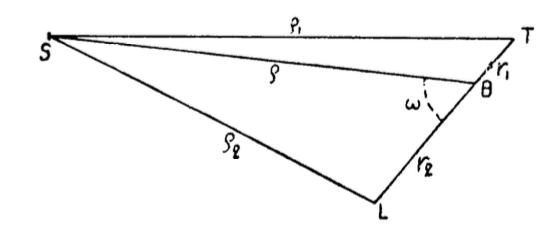
\includegraphics{21.png}
\end{center}

(Фиг 21)

Солнце S сообщает ускорения:
Земле: f * S/p12 по направлению TS
Луне: f * S/p22 > > LS

Вследствие чего точка (.) имеет ускорения:
T/T+L * f (S/q12) по направлению, параллельному TS
L/T+L * f (S/q22) > > > LS

Ускорения Солнца, происходящие от притяжения Земли и Луны, соответственно, суть:

f * (T/p12) по направлению ST
f * L/p22 > > SL

Поэтому ускорения точки (.) относительно точки S будут:

w1= f (S+T+L)/T+L * T/f12 по направлению параллельно TS

w2= f (S+T+L/T+L) * T/f22 > > > LS.

Разлагая эти ускорения, соответственно, по направлениям (.)S и (.)L, получим, как легко видеть из подобия показанных на фиг. 22 и 23 треугольников:
w11 = w1 * f/p2 по направлению (.)S
w1" = w1 * p1/f1 > > (.)L
w2' = w2 * f/f2  > > (.)L
W'2 = w2 * f/f1  > > (.)S
w2" = w2 * f2/p2 > > L(.)

\begin{center}
    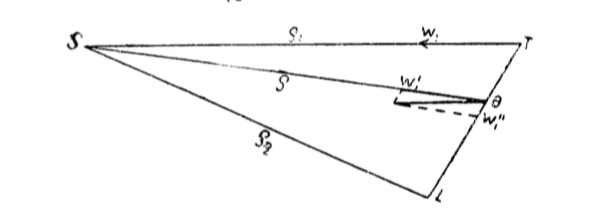
\includegraphics{22.png}
\end{center}
Фиг. 22.

Получим для ускорений точки (.) слагающие
W1 = w'2 + w'2 = f * (S+T+L)/T+L [ X * f/f3 + L]

\begin{center}
    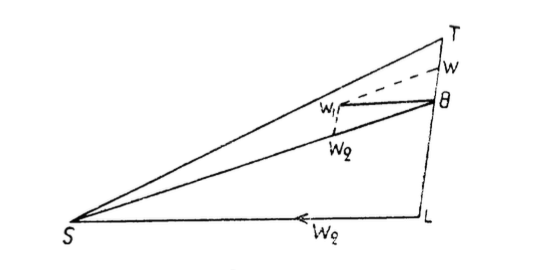
\includegraphics{23.png}
\end{center}
Фиг. 23.

\end{document}